% !TeX root = ../main.tex

\chapter{实验结果}\label{cha:experimetns}
本章中列出了VideoABC数据集上的大量的实验结果。首先,本文构建了一个人类水平测试的工具,用来检验人类在VideoABC数据集上的表现(第~\ref{sec:exp:humantest}~节);其次,第~\ref{sec:exp:results}~列出了VideoABC上不同模型的准确率,包括一些目前视频理解方面最先进的模型以及本文提出的HDR Net模型等等。在第~\ref{sec:exp:prob}~中,本文利用第~\ref{sec:abductive}~节中的概率模型来对VideoABC数据集进行检验,证明了观测信息起到了重要作用;最后,第~\ref{sec:exp:ablation}~列出了VideoABC和HDR Net 的一些消融实验的结果。

\section{人类水平测试工具}\label{sec:exp:humantest}
为了检验人类在VideoABC数据集的表现,本文开发了一个人类水平测试工具。与标注工具相同,这个测试工具也是以测试网站的形式实现的,所以可以满足多个测试人员同时答题。本节中将介绍这个测试工具的设计。测试界面如图~\ref{fig:humantest}~所示,整体界面非常简单。测试人员可以看到每个问题中的两个观测和四个假设选项,选中后点击提交按钮即可切换到下一题。
\begin{figure}[htbp]
    \centering
    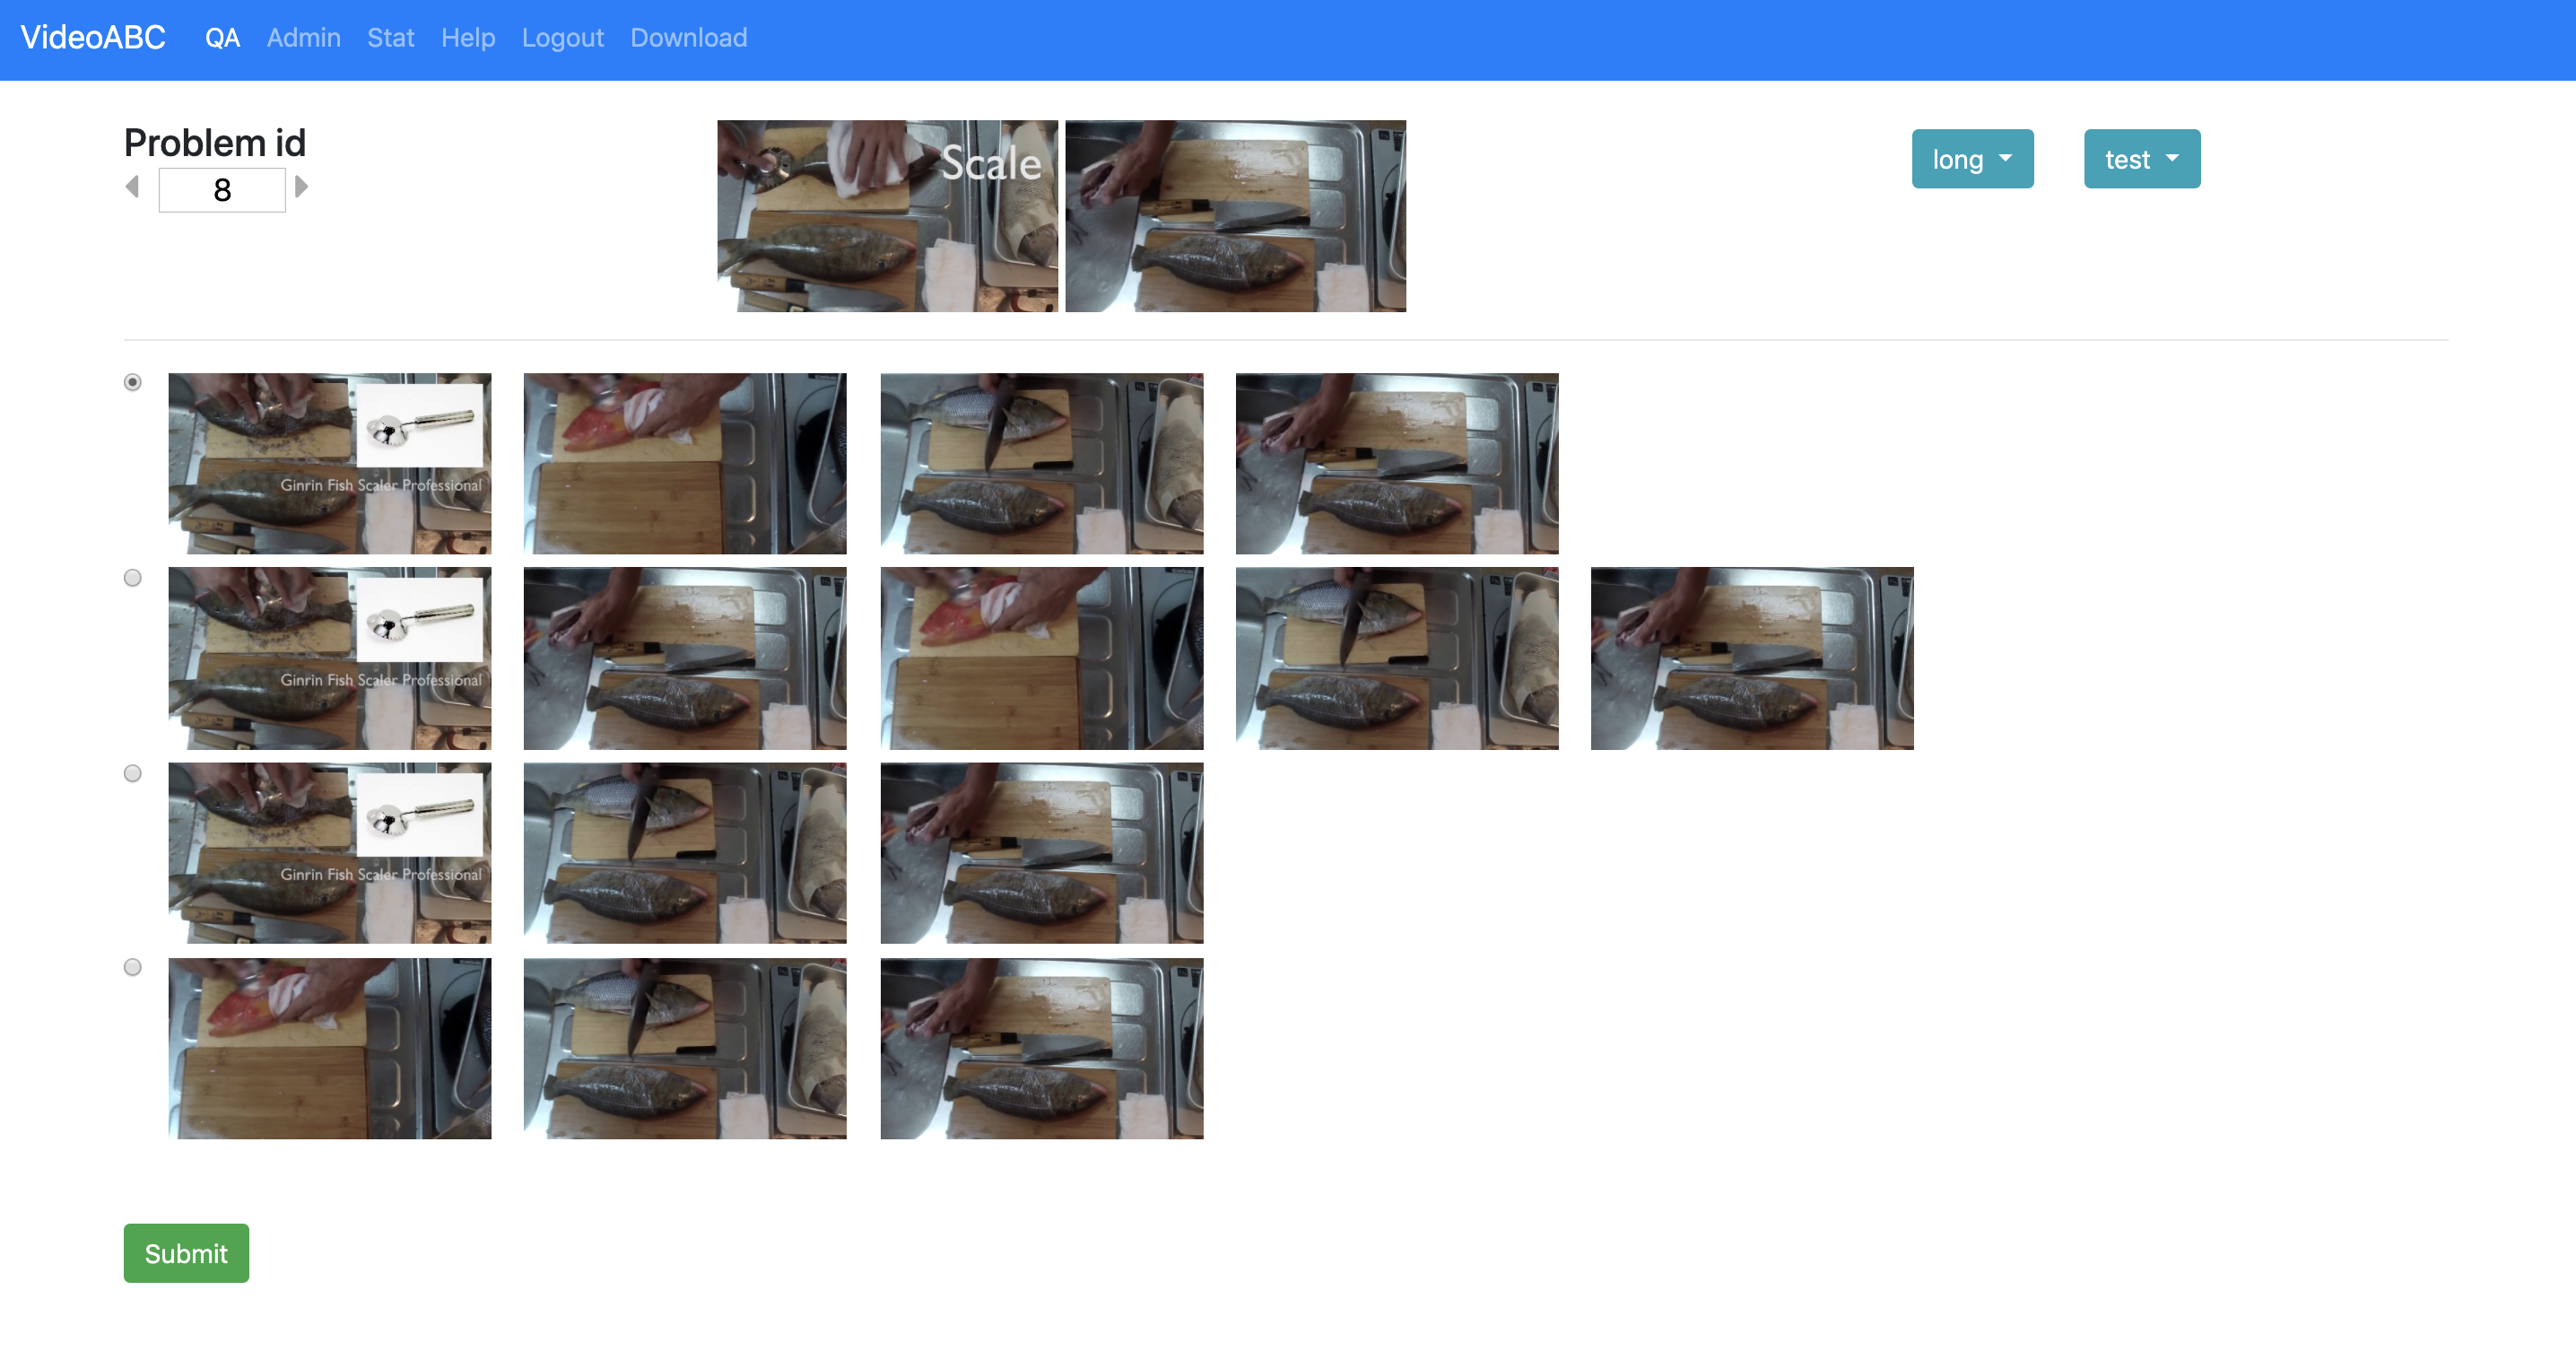
\includegraphics[width=\textwidth]{humantest.png}
    \caption{人类水平测试工具界面}
    \label{fig:humantest}
\end{figure}
测试工具的后端使用Django框架,前端使用Bootstrap框架。与标注工具不同的是,测试工具中需要记录每个测试者的成绩,所以需要设计注册和登录系统。注册和登录系统的界面如图~\ref{fig:sign}~所示。用户在访问标注工具时,必须先完成登录,若没有账号则需要注册一个账号。登录后,用户的信息会保存在cookie中,只要不登出就会始终保持登录状态。Django框架中内置了一套认证系统,包含了各种常见的账号操作,例如登录、登出、修改密码等等,编写代码时只需要完成与各个URL对应的HTML即可,Django 会自动完成与数据库的交互。登录操作则可以通过Django内置的用户表单类来实现。

\begin{figure}[htbp]
    \centering
    \begin{subfigure}{.5\textwidth}
        
\includegraphics[width=\textwidth{}]{signup.png}
        \caption{注册界面}
    \end{subfigure}%    
    \begin{subfigure}{.5\textwidth}
        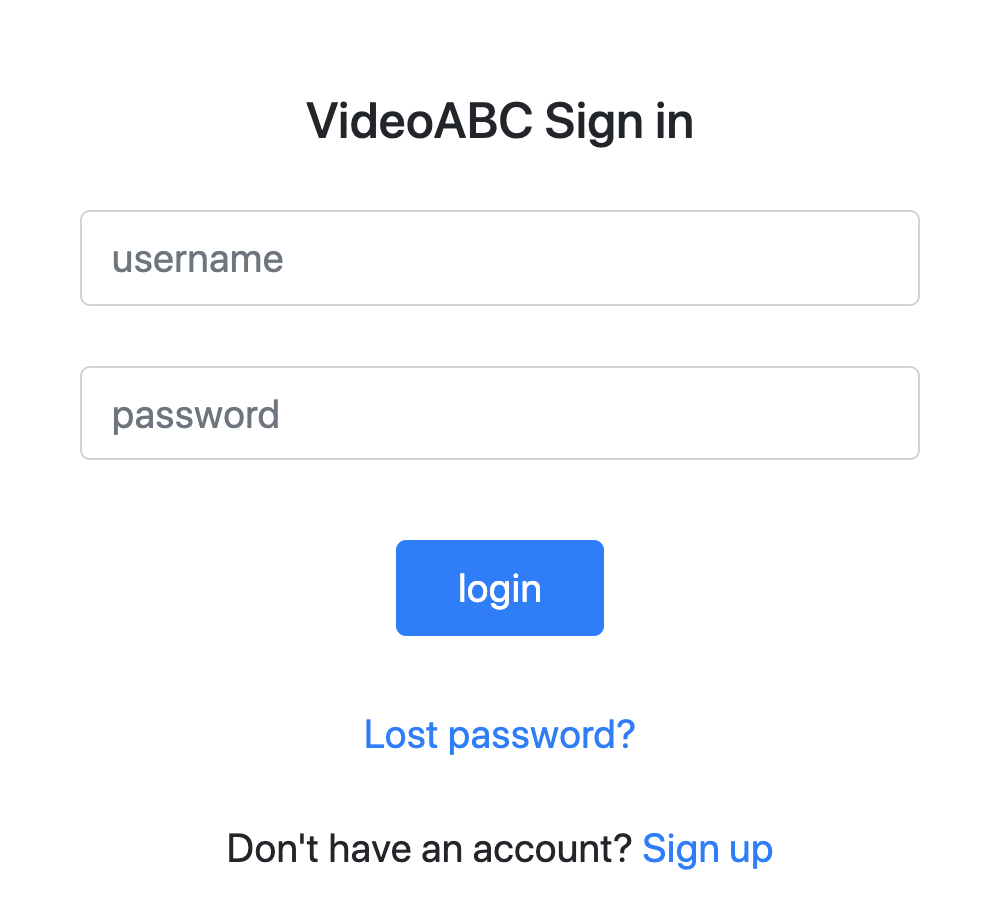
\includegraphics[width=\textwidth{}]{signin.png}
        \caption{登录界面}
    \end{subfigure}%
    \caption{注册和登录界面}
    \label{fig:sign}
\end{figure}

除了注册和登录功能之外,比较重要的部分就是数据结构的设计。测试工具中的一个基本的数据结构是Problem类,每个Problem对象表示一个问题,其主要成员变量如表~\ref{tab:problem}~所示。其中observation和hypothesis中存放的是图片的路径,不同的路径之间用逗号分隔;测试人员回答的答案以序号(0$\sim$3)保存。当测试人员提交答案时,该答案会添加到answers 中,而该用户的用户名会添加到answerers中,且保证顺序一致。答案保存后则从数据库中寻找该用户还没有回答过的问题,来作为该用户的下一个问题,这就保证了测试人员重复回答问题。

\begin{table}[htbp]
    \caption{Problem类主要成员变量}
    \label{tab:problem}
    \begin{tabu}to\textwidth{XXX}\toprule
        变量名称 & 变量类型 & 变量含义\\\midrule
        observation & 字符串 & 观测\\
        hypothesis & 字符串 & 假设\\
        answers & 字符串 & 回答\\
        answerers & 字符串 & 回答者\\
        correct\_answer & 小正整型 & 正确答案\\\bottomrule
    \end{tabu}
\end{table}

为了提高测试速度,测试工具中同样设计了快捷键,如表~\ref{tab:test_shortcut}~所示。同样,测试网站中也提供了帮助页面,便于测试人员明确答题规则。另外,测试网站的统计页面可以实时显示用户的答题准确率。

\begin{table}
    \caption{测试工具快捷键}
    \label{tab:test_shortcut}
    \begin{tabu}to\textwidth{XX}\toprule
        键盘按键 & 功能\\\midrule
        \keys{A}	& 选中选项A\\
        \keys{B}    & 选中选项B\\        
        \keys{C}	& 选中选项C\\
        \keys{D}    & 选中选项D\\
        \keys{Enter} & 提交答案\\\bottomrule
    \end{tabu}
\end{table}
\section{VideoABC上的实验结果}\label{sec:exp:results}

\subsection{实验模型}
为了测试不同模型在VideoABC数据集上的表现,本文测试了多种方法。
\paragraph{随机选择} 从所有的候选答案中随机选择一个,该结果可以用来检验数据集中的选项分布是否均匀。
\paragraph{TSN\cite{wang2016temporal}}TSN是一个简单的2D模型。TSN将视频均匀分割成几个片段,每个片段中抽取一帧,并使用2D卷积神经网络对这些帧提取特征,最后再通过一些运算将这些特征融合(取最大值、均值等等)。

\paragraph{TRN\cite{zhou2018temporal}} TRN是在TSN的基础上为了更好地对时序关系建模而提出的。TRN将TSN中特征合并的操作改成用关系网络(Relation Network)来实现,并通过多级的关系网络在不同的分辨率完成特征的融合。

\paragraph{R3D\cite{tran2018closer}} R3D是一个使用3D残差网络构建的视频理解模型。R3D将经典的2D Resnet 中的卷积换成3D卷积,能够很好地提取时空特征,在许多视频理解的任务中都取得了很好的结果。

\paragraph{R(2+1)D\cite{tran2018closer}} R(2+1)D是在R3D的基础上,将3D卷积分解成了空间上的2D卷积和时间上的1D卷积。在一些任务上,R(2+1)D的表现要比传统的3D卷积更好。

\paragraph{Non-Local Network\cite{wang2018non}} Non-Local Network 是以图像处理中的经典算法 Non-local means 的思路构建的一个模型,该模型能够捕捉时空上间隔较远的位置的关系。Non-local block 可以作为一个模块添加到其他的模型中,例如本文的实验中将该模块添加到R3D和R(2+1)D模型中。

\paragraph{HDR Net} 即本文提出的多级双重推理网络,详见第~\ref{cha:HDRNet}~章。
\subsection{实现细节}
对于TSN模型,本文使用BNInception的主干网络,与原文的实现\cite{wang2016temporal}保持一致。本文中将每个假设中所有步骤的图片放在一起构成一个视频,将其切分称$K=3$个片段,并从每个片段中抽取1帧,与两个观测一起作为TSN的输入。TSN中的特征融合方法采取了两种方法,即取最大值和取平均值。TRN的实现构建在TSN上,并使用多级融合的结构\cite{zhou2018temporal}。对于R3D和R(2+1)D,本文使用的pytorch官方的实现方式,以ResNet18\cite{he2016deep}为主干网络。本文提出的HDRNet中也使用ResNet18作为主干网络,这就保证了比较的公平性。由于每个假设中的步骤数目不同,实验时需要将所有的选项补零来保证每个选项的长度一致。在训练时 HDR Net的输入除了观测和假设,还包括每个假设的步骤数目,这样在用RNN完成推理过程的时候就可以跳过之前用于补零的步骤。在基于视频的模型中(R3D,R(2+1)D),最后的池化操作仅对有效的步骤长度取平均。对于2D的模型中(TSN,TRN),在加载数据的时候就只对有效步骤分段抽帧即可,不需要补零操作。对于人类水平的测试,本文列出了四位测试人员的平均准确率。

\subsection{实验结果}
表~\ref{tab:results}~展示了上文所述的不同方法的实验结果,以测试集上回答问题的准确率来衡量这些方法的表现。从中可以看到:

\begin{enumerate}
    \item 随机选择答案的准确率为25\%,说明了测试集中四个选项的分布比较均匀;
    \item 基于TSN的三种方法中,使用取平均值和取最大值融合的方法表现较差,与随机选择的准确率相差不大。使用关系网络(TRN)虽然有所提升,但准确度仍然很低。这说明基于2D卷积网络再进行特征融合的方法不适合VideoABC数据集;
    \item 基于视频的方法总体上表现较好。其中,R(2+1)D的准确率比R3D要高,说明将3D卷积分解为空间和时间上的卷积的做法有益于提取时空特征。另外,Non-Local模块也能一定程度上提升分类的准确率;
    \item 本文提出的HDR Net 在所有的模型上表现最好,超出其他最好的模型将近9个百分点。这是因为HDR Net专门为视频溯因常识推理任务而设计,能够成功地对步骤内和步骤间的时序关系建模;
    \item 人类的表现为92.4\%,远超其他所有的模型。这说明人类确实可以利用已有的常识取得比模型更好的表现。
\end{enumerate}

\begin{table}[htbp]
\caption{不同模型的在VideoABC上的准确率}   
\label{tab:results}
\begin{tabu}to\textwidth{XX}\\
\toprule
   模型/方法 & 准确率 (\%) \\
    \midrule
    Random & 25.0 \\
    \midrule
    TSN-\texttt{average}~\cite{wang2016temporal} & 24.9\\
    TSN-\texttt{max}~\cite{wang2016temporal} & 27.6\\
	TRN~\cite{zhou2018temporal} & 37.3\\
	\midrule
	R3D~\cite{R3D} & 73.1\\
	R(2+1)D~\cite{R3D} & 74.5\\
	R3D + Non-Local~\cite{wang2017non} & 74.3\\
	R(2+1)D + Non-Local ~\cite{wang2017non} & 76.0\\
	\midrule
	\textbf{HDR Net} & \textbf{85.2}\\
	\midrule
	Human & 92.4\\\bottomrule
    \end{tabu}
\end{table}

\section{消融实验}\label{sec:exp:ablation}
\subsection{步骤数目变化的影响}
在第~\ref{cha:VideoABC}~章中,本文介绍过VideoABC数据集的构建方式,在步骤切分和筛选的步骤中曾指定了最小步骤数$m=2$和最大步骤数$M=6$,本节中将探究不同步骤数对实验结果的影响。表~\ref{tab:VideoABC_steps}~列举了不同的配置以及命名。在这些配置中,$M$从1到6变化。由于需要保证$m\le M$,当$M=1$时,$m=1$。此时第~\ref{cha:VideoABC}~章中提到的错误选项类型中将不存在交换和删除,且正确选项中只包含一个步骤,推理时长较短,所以将其命名为short,意为短时推理(Short Time Reasoning, STR)。另外的几种配置则对应长时推理(Long Time Reasoning, LTR),对应着long2到long6的命名,其中的数字表示正确选项中的最大步骤数目$M$。需要注意的是,在LTR的任务中,所有选项的最长步骤应该为$M+1$(考虑到“插入”的错误类型)。与之前生成数据集的方式一样,表~\ref{tab:VideoABC_steps}~中不同配置的数据集也是经过难分选项挖掘的。图~\ref{fig:step_counts}~展示了不同步骤数配置的VideoABC数据集中的问题数,可见短时推理(short1)中的问题数目最多。这是因为任何一个单独的步骤都可以用来构成一个短时推理的问题,而在长时推理中需要将步骤数过少视频片段去除。

\begin{table}[htbp]
    \caption{不同最大步骤数的VideoABC数据集配置}
    \label{tab:VideoABC_steps}
    \begin{tabu}to\textwidth{XXX}\toprule
        最短步骤数$m$ & 最大步骤数$M$ & 名称\\\midrule
        1 & 1 & short\\\midrule
        2 & 2 & long2\\
        2 & 3 & long3\\
        2 & 4 & long4\\
        2 & 5 & long5\\
        2 & 6 & long6\\\bottomrule
    \end{tabu}
\end{table}

\begin{figure}
    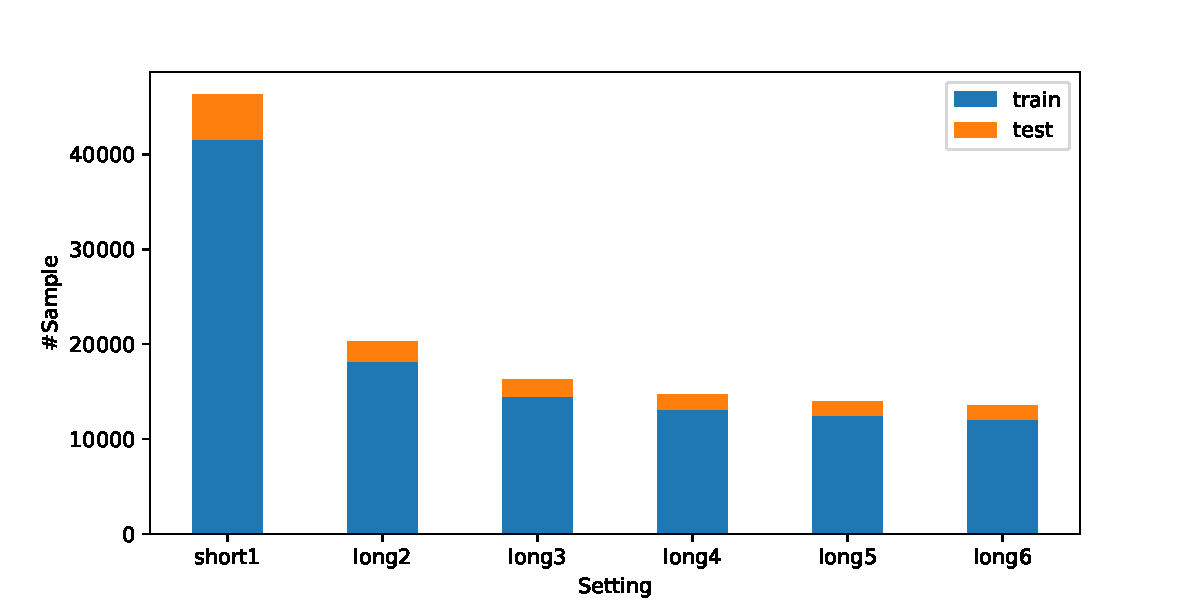
\includegraphics[width=\textwidth{}]{counts.pdf}
    \caption{不同步骤数配置的VideoABC中的问题数}
    \label{fig:step_counts}
\end{figure}

表~\ref{tab:result_steps}~展示了不同最长步骤数$M$的实验结果。可以看到总体上来说,随着$M$的增加,各种方法的分类准确率逐渐降低。这说明了$M$越大,模型越需要适应更大变化范围的步骤数目,从而推理的难度就越大。基于这个结论,本文将其中最难的,即$M$最大的配置作为标准的VideoABC数据集配置,用来检验不同模型完成视频溯因常识推理任务的能力。
\begin{table}
    \caption{不同最长步骤数的实验结果}
    \label{tab:result_steps}
    \begin{tabu}to \textwidth{l*{6}{X[c]}}\\
        \toprule
            \multirow{2}{*}{方法} &\multicolumn{6}{c}{数据集配置}\\\cmidrule{2-7}
            & short & long2 & long3 & long4 & long5 & long6\\
            \midrule
        Random & 25.0 & 25.0 & 25.0 & 25.0 & 25.0 & 25.0\\
         \midrule
        TSN-\texttt{average} & 30.2 & 18.3 & 15.3 & 17.1 & 14.6 & 16.4 \\
        TSN-\texttt{max} & 24.1 & 26.4 & 29.3 & 27.6 & 26.9 & 28.6 \\
         \midrule
        R3D & 84.7 & 85.5 & 79.1 & 74.4 & 73.9 & 73.1 \\
        R(2+1)D & 86.9 & 86.8 & 81.6 & 74.4 & 74.4 & 74.5 \\
         \bottomrule
        \end{tabu}
\end{table}

\subsection{难分样本挖掘的效果}
为了去除每个问题中过于显然的假设,提高数据集的难度VideoABC构建的步骤中包括了难分样本挖掘这一步骤,本节中将检验这操作的效果。表~\ref{tab:hard_mining}~中列举了难分样本挖掘前后R3D~\cite{tran2018closer}模型的准确率,可见在所有的数据集配置下,模型的准确率经过难分样本挖掘的步骤后都降低了很多。这说明了难分样本挖掘的步骤确实可以提高数据集的难度,从而能够更好地检验模型的推理能力。

\begin{table}
\caption{难分样本挖掘前后的准确率}
\label{tab:hard_mining}
\begin{tabu}to\textwidth{l*{2}{X[c]}}\toprule
\multirow{2}{*}{数据集配置} & \multicolumn{2}{c}{难分样本挖掘}\\\cmidrule{2-3}
&\xmark&\cmark\\\midrule
short1 & 90.0 & 84.7 \\
long2 & 94.0 & 85.5\\
long3 & 86.1 & 79.1\\
long4 & 82.3 & 74.4\\
long5 & 83.9 & 73.9\\
long6 & 78.7 & 73.1\\\bottomrule
\end{tabu}
\end{table}

\subsection{网络结构和大小的影响}
从表~\ref{sec:exp:results}~可以看到,表现较好的几个模型都是以3D残差网络(R3D)或类似的结构为主干网络的。本节中将以R3D为基础,探究不同网络结构和网络大小的影响,如表~\ref{tab:arch}~所示。其中R3D是以ResNet18为基础,将2D卷积换成3D卷积实现的;R(2+1)D则是将3D卷积分解成空间上(2D)和时间上(1D)的卷积;另一种结构变化是在R3D中加入Non-Local block\cite{wang2018non};最后列出了34层的R3D的结果。可以看到,改变网络结构对准确率的影响并不大,即使是34层的网络,比18层的也仅仅多出1.8\%。另一方面,本文提出的HDRNet模型在保持主干网络只有18层的基础上,通过引入推理模块达到了85.2\%的准确率,远超其他的模型。

\begin{table}[!h]
\caption{不同网络结构和大小的影响}
\label{tab:arch}
\begin{tabu}to\textwidth{XXX}\toprule
    模型结构 & 层数 & 准确率\\\midrule
    R3D & 18 & 73.1\\
    R(2+1)D & 18 & 74.5\\
    R3D + Non-local & 18 & 74.3\\\midrule
    R3D & 34 & 74.9\\\midrule
    \textbf{HDRNet} & 18 & \textbf{85.2}\\\bottomrule
\end{tabu}
\end{table}

\section{概率模型检验}\label{sec:exp:prob}
VideoABC数据集的一个特点在于,模型必须对两个观测有全面的理解才能选出正确的答案,而不能只从选项中通过一些捷径判断。为了验证观测信息的重要性,本文利用第~\ref{sec:abductive}~节中介绍过的概率模型来对VideoABC数据集进行实验。本节中使用的网络为R3D\cite{tran2018closer},故输入应该是视频的形式。在具体实现的过程中,输入的视频是由可用信息按照时序关系进行拼接实现的。根据不同的概率模型,具体的输入形式也有所不同,如表~\ref{tab:input_formt}~所示,其中的概率模型和简称与第~\ref{cha:vacr}~中介绍的相同。在VideoABC数据集中,每个假设$H_i$由一系列步骤构成,每个步骤是一个视频片段,所以这里输入的每个$H_i$是多个步骤的视频片段拼接而成。这里需要注意的是,为了实现线性连的结构需要训练两个模型(见式~\eqref{equ:LC}~)。

\begin{table}
\caption{不同概率模型的输入形式}
\label{tab:input_format}
\begin{tabu}to \textwidth {XXX[2]}\\\toprule
    概率模型 & 简称 & 输入形式\\
    \midrule
    仅假设 & HO & $H_i$\\
    仅第一个观测 & 1st-OO & concat($H_i$, $O_1$)\\
    仅第二个观测 & 2nd-OO  & concat($H_i$, $O_2$)\\
    线性链 & LC & concat($H_i$, $O_1$); concat($H_i$, $O_1$)\\
    全连接 & FC & concat($H_i$, $O_1$, $O_2$)\\     \bottomrule
\end{tabu}
\end{table}

\begin{table}[!h]
\label{tab:prob}
\begin{tabu}to \textwidth {XXX}\\
\toprule
   概率模型 & STR & LTR \\
    \midrule
     HO  & 25.2 & 56.6\\
     1st-OO & 70.1 & 67.3\\
     2nd-OO & 79.1 & 69.9\\
     LC & 82.9 & 71.9\\
     FC & 84.7 & 73.1\\  
 \bottomrule
\end{tabu}
\end{table}
表~\ref{tab:prob}~展示了不同概率模型在短时推理(STR,对应配置为short1)和长时推理(LTR,对应配置为long6)任务上的表现。从表中可以看出,输入中仅仅包含假设的模型准确率最低,随着概率模型中的连接数增多,准确率也逐渐提高。总体上来说,模型在LTR任务上的准确率要低于STR上的准确率,但是对于HO的概率模型情况正好相反。这是因为在STR任务中,各个假设都是不同的单个步骤,所以仅仅通过假设是不可能得出正确答案的;而在LTR任务中,模型可以通过判断每个选项内部的时序先后关系来给出答案,但是这种方法在处理某些错误类型时可能并不会起到很好的效果,例如错误类型“删除”并没有改变时序的先后关系。所以,虽然HO概率模型在LTR中的准确率比STR高,但是仍然与全连接概率模型相比有很大的差别。从这一系列实验中可以看出,要想在VideoABC数据集中取得较高的准确率,必须充分利用两个观测的信息完成推理,这也从另一方面验证了VideoABC数据集的合理性。

